The number of parallel connections refers to a browser's ability to establish simultaneous connections to retrieve 
multiple resources concurrently. Increasing parallel connections can potentially expedite page load times, but it may 
also strain server resources and lead to network congestion. Specifically:

\begin{itemize}[leftmargin=10pt]
\item \textbf{Fewer Parallel Connections}: If the number of parallel connections is set too low, it can result in
 slower page load times. With fewer connections, the browser fetches resources sequentially, causing delays as it waits
 for each request to complete before initiating the next one.
\item \textbf{Default Number of Parallel Connections}: Most modern browsers allow around six parallel connections per
 host by default. This number hit a balance between resource fetching and the server's load. With this setting, the 
 browser can fetch multiple resources simultaneously, improving the overall page load performance. 
\item \textbf{Higher Number of Parallel Connections}: Increasing the number of parallel connections can potentially
 speed up page load times. By allowing more simultaneous connections, the browser can fetch a greater number of 
 resources in parallel, reducing the overall loading time. However, an excessively high value may overwhelm the 
 server and cause network congestion.
\end{itemize}
\noindent
This section presents a practical investigation into the influence of the number of parallel connections on the Page Load Time (PLT). 
Various websites (as listed in Table \ref{tab:websites_details}) were tested using different numbers of parallel connections 
to determine the configurations that benefit the most from parallel TCP connections.

    \begin{table}[H]
        \small
    \centering
    \rowcolors{2}{pyblue!25}{white}
        \begin{tabular}{|l|c|c|}
        \hline
        \rowcolor{pyblue!60}
        \textbf{Website} & \textbf{Number of Objects} & \textbf{Size (MB)} \\
        \hline
        Vallesabbia & 118 & 5.01 \\
        Grafiche & 65 & 5.31 \\
        Vallespluga & 151 & 20.03 \\
        Unitus & 72 & 1.74 \\
        Gov & 218 & 9.98 \\
        Istat & 134 & 11.33 \\
        \hline
        \end{tabular}
        \caption{\small Websites details}
        \label{tab:websites_details}
    \end{table}


Before each measurement, the browser cache was cleared and the "disable cache" option in Mozilla Web Developer Tools was enabled. 
The selection of tested sites was conducted carefully to utilize the HTTP/1.1 protocol, which allows for the utilization of multiple parallel TCP connections. 
This choice aimed to highlight the potential benefits that can be derived from employing such connections. Each website was tested using different numbers of 
TCP connections, specifically 1, 5, 10, and 15. To ensure accurate measurements, the reported Page Load Time (PLT) represents the average value obtained 
from five data points collected under the same experimental conditions.
It is important to note that the actual number of TCP connections established depends on the server configuration, as the client merely expresses its preference. 
To ensure proper interpretation of the results, the number of opened TCP connections was verified using Wireshark, and these details are provided 
in Table \ref{tab:TCP_asked}.

    \begin{table}[H]
        \small
    \centering
    \rowcolors{2}{pyblue!25}{white}
        \begin{tabular}{|l|c|c|}
        \hline
        \rowcolor{pyblue!60}
        \textbf{Website} & \textbf{N. TCPs Ask} & \textbf{N. TCPs Estab.} \\
        \hline
        Vallesabbia & 15 & 15 \\
        Grafiche & 15 & 13 \\
        Vallespluga & 15 & 15 \\
        Unitus & 15 & 15 \\
        Gov & 15 & 15 \\
        Istat & 15 & 15 \\
        \hline
        \end{tabular}
        \caption{\small Number of TCP connections asked and established}
        \label{tab:TCP_asked}
    \end{table}

Analysis of Figure \ref{fig:plt_n_tcp} reveals a decrease in PLT as the number of connections increases. However, this trend only persists until a certain threshold 
(in this case, 5 connections), beyond which the PLT remains relatively constant. The specific reasons for this behavior are not apparent from the conducted 
experiments, as the servers configuration remains unknown, resembling a black box. Notably, the website that derives the most benefit from concurrent TCP 
connections is \textit{Istat}. This advantage is not solely attributable to the size of the website or the number of objects it contains, as other 
websites with larger sizes exhibit a different behavior. Therefore, further investigations are necessary to identify the underlying factors contributing 
to this phenomenon.
Overall, it can be concluded that the number of parallel TCP connections significantly impacts the PLT. However, the benefits tend to plateau as the number of 
connections increases excessively. The default choice of six concurrent TCP connections made by the browser appears to be a reasonable selection based on the 
findings of this study.
    
    \begin{figure}[H]
        \centering
        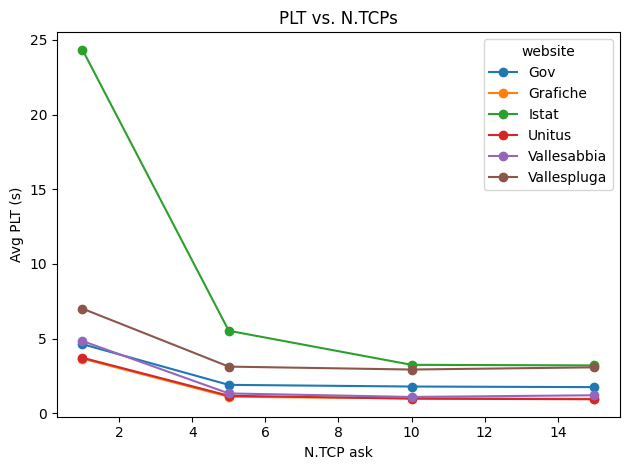
\includegraphics[width=0.48\textwidth]{1_plt_n_tcp.png}
        \caption{\small Page Load Time (PLT) vs. N.TCP}
        \label{fig:plt_n_tcp}
    \end{figure}



